%\thispagestyle{myheadings}
\section{Invited Talk: Gideon Mann}
\index{Mann, Gideon}

\begin{center}
\begin{Large}
    {\bfseries\Large Understanding the News that Moves Markets} \vspace{1em}\par
\end{Large}

%% \begin{center}
%%   \begin{tabular}{m{1in}b{1in}}
%%     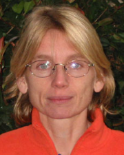
\includegraphics[width=1in]{content/monday/cortes-headshot.png}
%%     & {\bfseries Corinna Cortes} \newline Google Research, NY
%%   \end{tabular}
%% \end{center}

\daydateyear, 9:00--10:00 \vspace{1em}\\
\PlenaryLoc \\
\vspace{1em}\par
%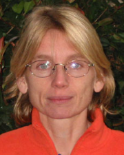
\includegraphics[height=100px]{content/monday/cortes-headshot.png}
\end{center}

\noindent
{\bfseries Abstract:} Since the dawn of human civilization, finance and language technology have been connected. However, only recently have advances in statistical language understanding, and an ever-increasing thirst for market advantage, led to the widespread application of natural language technology across the global capital markets. This talk will review the ways in which language technology is enabling market participants to quickly understand and respond to major world events and breaking business news. It will outline the state of the art in applications of NLP to finance and highlight open problems that are being addressed by emerging research.
\vspace{3em}\par 

\vfill
\noindent

{\bfseries Biography:} Gideon Mann is the Head of Data Science at Bloomberg L.P., where he guides the strategic direction for machine learning, natural language processing (NLP) and search across the company. He is part of the leadership team for the Office of the CTO. He served as a founding member of both the Data for Good Exchange (D4GX), an annual conference on data science applications for social good, and the Shift Commission on Work, Workers and Technology. He has also been active in academic research in fact extraction, weakly-supervised learning, and distributed optimization. Recently, he has also been interested in applications of machine learning to problems in software engineering. From 2007 to 2014, he worked at Google Research in New York City, and his team built core machine learning libraries, released the Google Prediction API, and developed Colaboratory. Mann graduated Brown University in 1999 and received a Ph.D. from The Johns Hopkins University in 2006.

\newpage
